\chapter{Microseq}
\section{Introductory Reading}

\nomenclature{Glossary term:}{Definition}

The conversion of working DNA to proteins is one of the most important processes in biology.
After DNA undergoes transcription and becomes an mRNA sequence, it can be turned into a string of amino acids via sequences known as codons.
Each codon consists of a combination of three nucleotides, and there are twenty amino acids that match with these combinations.

DNA and all DNA processes are integral to scientists' understanding of biology.
Studying this molecule is a fascinating and essential task, but because of the large quantities of data that genetics studies can obtain, manually analyzing a sequence can prove to be insignificant.
Bioinformatics is a relatively recent field that combines computational science, statistics, engineering, and biology in order to interpret this type of data.
Being able to use technology to aid in the analysis of different sequences can greatly lessen the tediousness of translating sequences and manually visualizing data.
It also eliminates the possibility of human error, and allows genetics research to move much faster.

For example, existing algorithms, such as JASPAR and STARR-seq, are databases or functional tools that allow bioinformaticians to analyze sequence data.
These programs can do things such as identify even remotely homologous sequences from a DNA multiple sequence alignment, or identify \textit{cis-}regulatory regions throughout the genome.\cite{jaspar} 
The focus of this case study are R packages known as Biostrings and microseq, which, in conjuction, allow for sequence data analysis. 

\section{Objectives of the Case Study}

The objective of this study is to use the Biostrings and microseq packages in conjunction to translate a plain sequence format of DNA.

\subsection{Objective 1}

Translation of DNA to RNA is a vital biological process, and using the Biostrings and microseq functions will allow for a significantly streamlined process that will aid projects or studies in need of translated DNA.
The objective is to obtqain an amino acid sequence translated automatically from the given DNA sequence.


\section{Building the Model}

Tips for building the model are located in the comment sections of the code.

If the code is written properly, the output should be a list with the frequencies of each amino acid in the DNA sequence.
The output should look similar to figure \ref{fig:aminofreq}.

\begin{figure}[htbp!] %  the "H" means put it where you put this code....but that doesn't always work!
   \centering
   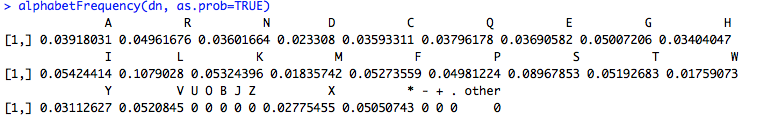
\includegraphics[width = \textwidth]{pictures/microseq/screenshot.png} 
   \caption{Frequency of amino acids}
   \label{fig:aminofreq}
\end{figure}

\section{Deliverable}

The student should submit a list containing the frequencies of each amino acid in the sequence analyzed.
This list can be compared to the instructor's frequencies list to check for accuracy.

\section{Teaching Code}

You should also put any notes, teaching suggestions, etc. in this space!


\begin{lstlisting}
# Name
# Date
# Name of script
# Objective of script

# clean up and set working directory
rm(list=ls()) 
setwd()

### download data set from
ftp://ftp.ensembl.org/pub/release-85/fasta/mus_musculus/dna/

### install Biostrings from
https://bioconductor.org/packages/release/bioc/html/Biostrings.html
### then install microseq

#load  microseq and Biostrings library
library()
library()

# view accepted IUPAC DNA letters
# these are the values that the functions will accept and put out
DNA_BASES
DNA_ALPHABET

# obtain plain sequence format from .txt file on desktop or source
# turn fasta into string
d <- readDNAStringSet("data set")
# translate object to amino acid sequence
dn <- translate(data set, genetic.code=GENETIC_CODE, if.fuzzy.codon = "solve") 
#"solve" allows unidentifiable codons to be represented as *

#characteristics of DNA strings
d
summary(data set)
dn
summary(translated data set)

#frequency of each letter or present symbol
alphabetFrequency(translated data set)

#frequency values
alphabetFrequency(translated data set, as.prob=TRUE)

### EXTRA CREDIT!
letterFrequency(translated data set, "A", as.prob=TRUE)
letterFrequency(data set[[1]], letters="ACGT", OR=0)

# What do these two functions show? 
#show frequency of base "A" in translated data set, and quantity of "ACGT" in
original data set
\end{lstlisting}

\section{Example Student Code}

\begin{lstlisting}
# Christa Parrish
# September 8, 2016
# translate.R
# this script translates DNA sequence to Amino Acid sequence and observes frequencies 
of letters

# clean up and set working directory
rm(list=ls())
setwd("~/Desktop/R")

### download data set from ftp://ftp.ensembl.org/pub/release-85/fasta/mus_musculus/dna/

#load  microseq and Biostrings library
library(microseq)
library(Biostrings)

#view accepted IUPAC DNA letters
DNA_BASES
DNA_ALPHABET

# obtain plain sequence format from .txt file on desktop or source, whichever works
# turn fasta into object
d <- readDNAStringSet("MusMusculus.fa")
# translate object
dn <- translate(d, genetic.code=GENETIC_CODE, if.fuzzy.codon = "solve") 
#"solve" allows unidentifiable codons to be represented as *

#characteristics of DNA strings
d
summary(d)
dn
summary(dn)

#frequency of each letter or present symbol
alphabetFrequency(dn)

#frequency values
alphabetFrequency(dn, as.prob=TRUE)

### EXTRA CREDIT!
letterFrequency(dn, "A", as.prob=TRUE)
letterFrequency(d[[1]], letters="ACGT", OR=0)

# What do these two functions show?
\end{lstlisting}


\section{Further Readings}

By looking at the package manual online, students can read about the other functions of the microseq and Biostrings packages.

\printnomenclature
